\subsection{Dataset}
\label{sec:dataset}

Este proyecto empleará el dataset denominado \textit{Brain Tumor MRI Datasets}, disponible públicamente en la plataforma Kaggle y publicado por Shashin \cite{Shashin2024}. Este conjunto de datos comprende 8764 imágenes de resonancia magnética cerebral estructuradas para una tarea de categorización binaria.

Las imágenes se encuentran organizadas en dos categorías: Yes (sujetos que presentan tumor cerebral) y No (sujetos sin hallazgos tumorales).

\begin{figure}[H]
\centering
\begin{minipage}{0.34\textwidth}
    \centering
    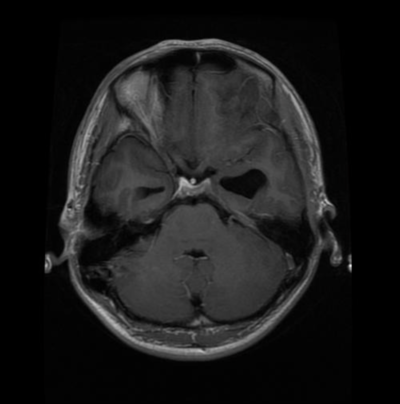
\includegraphics[width=\textwidth]{images/Si_Tumor.png}\par
    \caption{Ejemplar de imagen de la categoría ``Yes''.}
    \label{fig:si_tumor}
\end{minipage}

\vspace{0.3cm}

\begin{minipage}{0.34\textwidth}
    \centering
    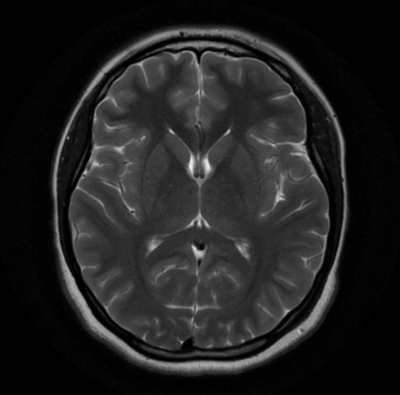
\includegraphics[width=\textwidth]{images/No_Tumor.png}
    \caption{Ejemplar de imagen de la categoría ``No''.}
    \label{fig:no_tumor}
\end{minipage}
\end{figure}

El conjunto se encuentra particionado en un 80\% destinado a entrenamiento y un 20\% reservado para validación, estrategia que facilita el desarrollo y la valoración de modelos de aprendizaje profundo. Considerando que se trata de un dataset de imágenes, carece de atributos tabulares convencionales; cada registro se compone de una imagen de resonancia magnética acompañada de su correspondiente etiqueta categórica.

\begin{table}[H]
\centering
\caption{Des\-crip\-ción de las variables del dataset.}
\label{tab:variables}
\begin{tabular}{lp{0.65\columnwidth}}
\hline
Variable & Descripción \\
\hline
Imagen MRI & Imagen de resonancia magnética cerebral. \\
Clase      & Etiqueta de la imagen (``Yes'' o ``No''). \\
Train/Test & Indica si la imagen pertenece al conjunto de entrenamiento o de prueba. \\
\hline
\end{tabular}
\end{table}

La estructura del conjunto de datos se organiza en dos subgrupos distintos: entrenamiento y prueba. La caracterización del volumen de imágenes según categoría se presenta en la Tabla~\ref{tab:distribucion}.

\begin{table}[H]
\centering
\caption{Distribución de imágenes por clase y conjunto.}
\label{tab:distribucion}
\begin{tabular}{lrrr}
\hline
Conjunto & No Tumor & Tumor & Total \\
\hline
Train     & 2869 & 4143 & 7012 \\
Test      &  717 & 1035 & 1752 \\
Total & 3586 & 5178 & 8764 \\
\hline
\end{tabular}
\end{table}

Con propósito de caracterizar la composición del conjunto, se efectuó un análisis considerando la cantidad de ejemplares por categoría y por partición.

\begin{figure}[H]
\centering
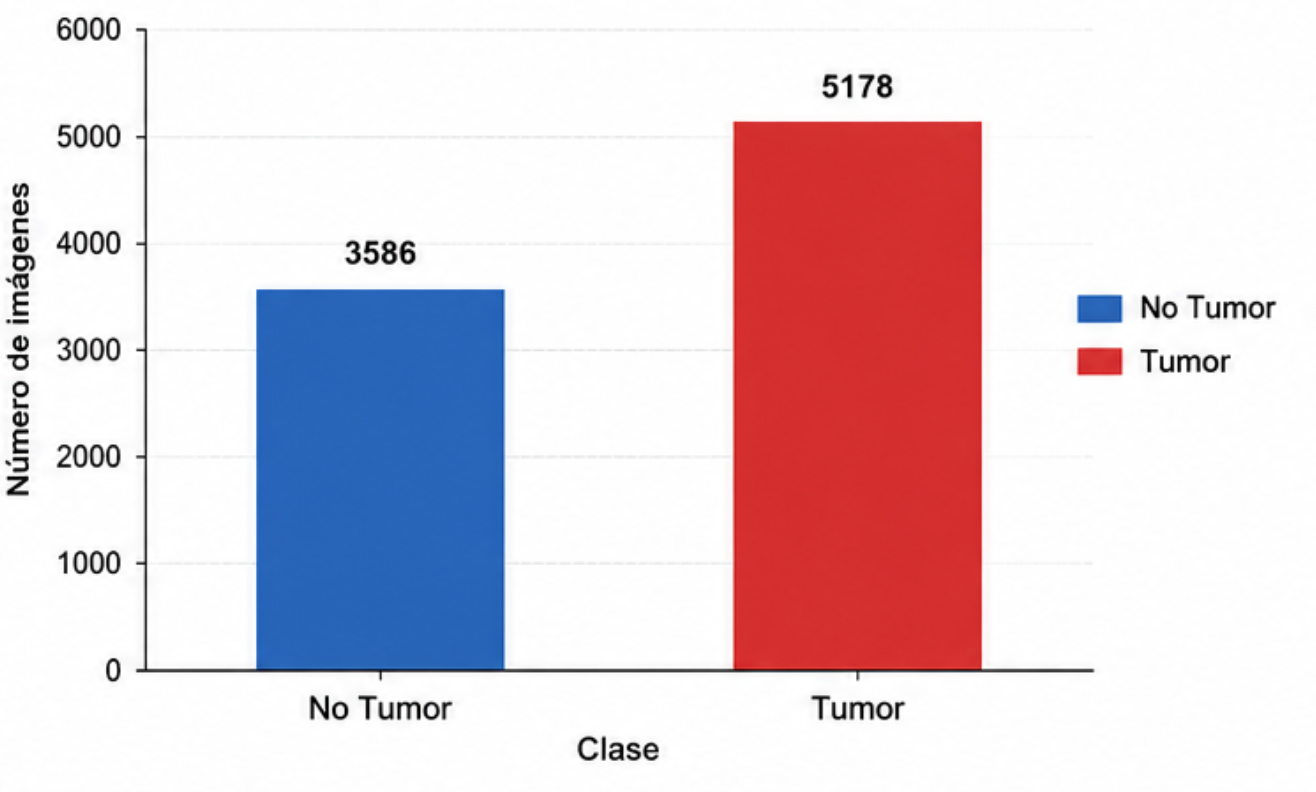
\includegraphics[width=0.4\textwidth]{images/Distribucion_De_Imagenes_por_Clases.png}
\caption{Distribución total de imágenes por clase.}
\label{fig:dist_clases}
\end{figure}

Según se observa en la Figura~\ref{fig:dist_clases}, el conjunto contiene 5178 imágenes con tumor (59.1\%) y 3586 imágenes sin tumor (40.9\%). Esto indica un ligero desequilibrio entre categorías, aunque la magnitud de la diferencia no resulta lo suficientemente pronunciada para comprometer significativamente el entrenamiento.

\begin{figure}[H]
\centering
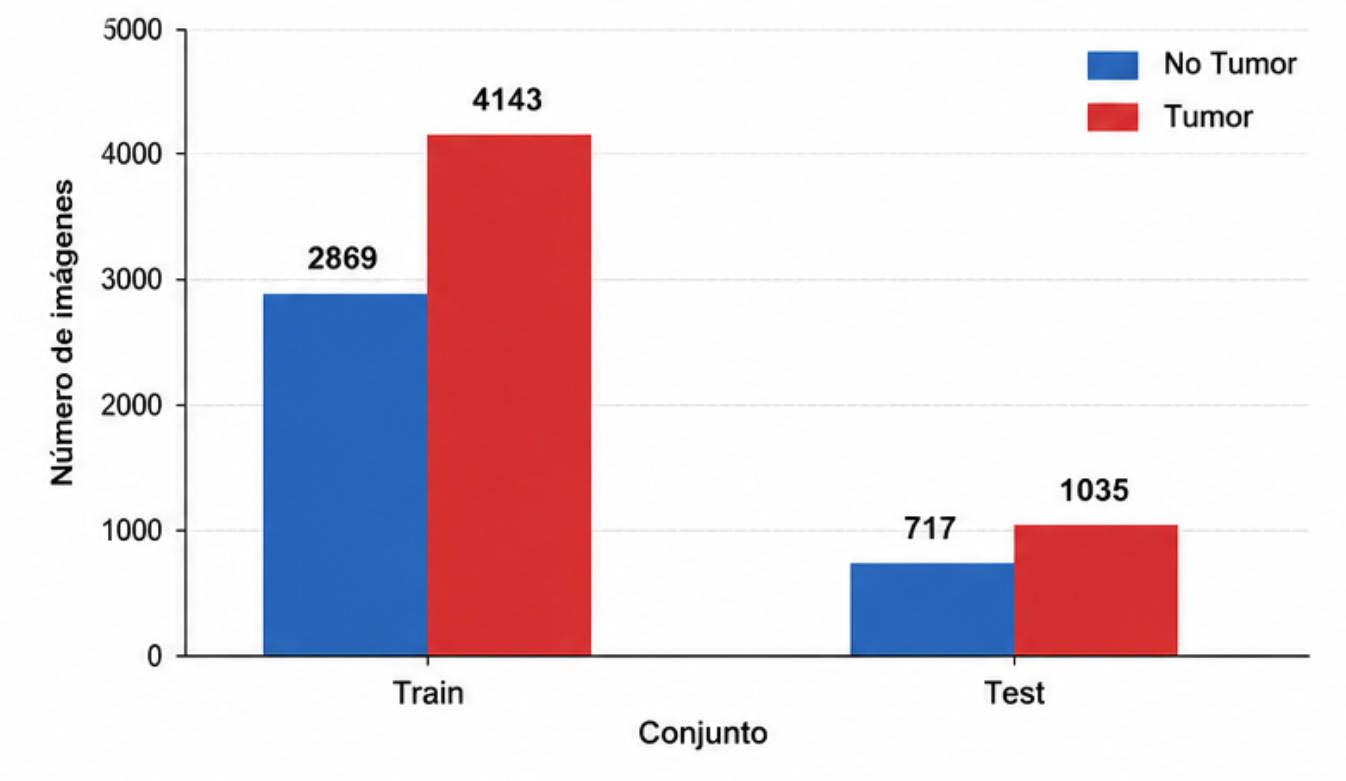
\includegraphics[width=0.4\textwidth]{images/Distribucion_De_Imagenes_por_clase_y_conjunto.png}
\caption{Distribución de imágenes por conjunto de entrenamiento y prueba.}
\label{fig:dist_conjunto}
\end{figure}

La Figura~\ref{fig:dist_conjunto} ilustra que la proporción de imágenes se mantiene consistente tanto en el subgrupo de entrenamiento como en el de prueba. En ambas particiones, la categoría Tumor exhibe una cantidad superior de muestras comparada con la categoría No Tumor, preservando una relación proporcional equiparable entre ambos subconjuntos.

\begin{figure}[H]
\centering
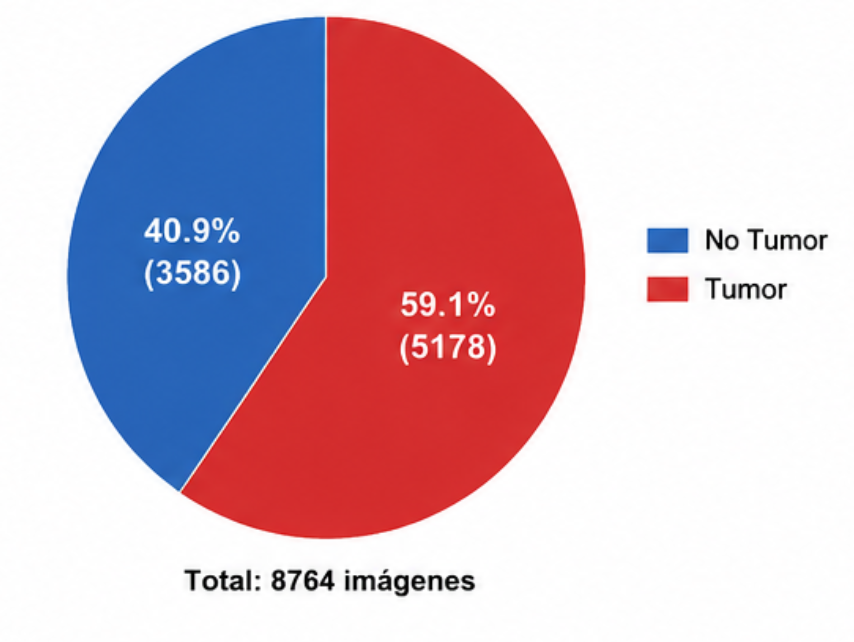
\includegraphics[width=0.3\textwidth]{images/Distribucion_porcentual_Por_Clase.png}
\caption{Distribución porcentual de las clases del dataset.}
\label{fig:dist_porcentual}
\end{figure}

La Figura~\ref{fig:dist_porcentual} presenta la distribución porcentual de los ejemplares del dataset. Se aprecia que el 59.1\% corresponde a imágenes que presentan tumor cerebral, en tanto que el 40.9\% pertenece a imágenes sin tumor. Este diferencial revela un desequilibrio moderado entre categorías que requiere consideración durante las fases de entrenamiento.
